\documentclass[a4paper,12pt]{article}
\usepackage[utf8]{inputenc}
\usepackage{graphicx} % Required for inserting images
\usepackage{amsmath}
\usepackage{amssymb}

\usepackage[left=2cm, right=2cm, top=2cm, bottom=2cm]{geometry}
\usepackage[greek,english]{babel}
\usepackage{tikz}
\usetikzlibrary{positioning,fit,arrows.meta} 

\title{Trait evolution in a mutualistic network}

\begin{document}

\maketitle

Let $P_{t,i}$ be the number of plants of species $i$ at time $t$ and $A_{t,i}$ the number of animals (pollinators) of species $j$. Let $\mu_{P_i}$ and $\mu_{A_j}$ be the mean trait of plant species $i$ and animal species $j$. The animal trait is the proboscis length and the plant trait is the corolla length. I propose the following population dynamic model, based on the Ricker model: 

\begin{align}
    P_{t+1,i} = P_{t,i} e^{r_{P_i} + B_{P_i} - C_{P_i} - m_{P_i} P_{t,i}} \label{pop_dyn_P}\\
    A_{t+1,j} = A_{t,j} e^{B_{A_j} - C_{A_j}  \label{pop_dyn_A}}
\end{align}

The exponent in the Ricker model consists of the per individual net growth rate. In the original Ricker model this was simple negative density dependence $r(1 - \frac{N}{K})$ where $N$ is population size and $r$ and $K$ are the intrinsic growth rate and carrying capacity, respectively. Here, we model the net growth rate as the difference between a reproduction (benefits $B$) term, which depends on the nectar consumed (animals) or pollination service received (plants) via a Monod equation (see below), and a cost term ($C$) for the nectar production (plants). There is no cost to the mutualistic interaction for animals, but there are costs associated with the proboscis (see below). For the plants we also include an intrinsic growth rate $r_{P_i}$ which is also present in absence of pollinators (but it could be set equal to 0 for obligatory mutualistic interactions), and costs due to competition for other resources (water, light, space) that increase density-dependent mortality (mortality term ($m_{P_i}$)). This will prevent the population size of plants to explode as it receives more and more services as the animal population grows. For the animals we do not add these two terms, as we assume that nectar consumption is obligatory and also the resource for which they compete. Their population sizes will be limited by limitation on the plant population sizes. Let us focus first on the costs for the animals, where the larger the proboscis, the higher the costs invested in maintaining the proboscis and the energy needed for movement. We model this as follows:

\begin{align}
    C_{A_j} = C_{A_0} e^{\frac{\mu_{A_j}}{\mu_{A_0}}}
    \label{Animal_costs}
\end{align}

\noindent where $\mu_{A_0}$ controls how fast the mortality rate (costs) increase with the mean trait value. For the plants, the costs are not so much in the maintenance of the corolla, but in the nectar that needs to be produced. We assume that each visit of animals results in nectar consumption and hence the costs, $C = C^\mathrm{prop}$ are proportional to the pollinators that have a matching proboscis (similar to the model by Holland \& DeAngelis (2010) with a very large half-saturation constant):

\begin{align}
    C^\mathrm{prop}_{P_i} = c \sum^{S_A}_{j = 1} M^C_{A_{j,i}}
\end{align}

\noindent with $c_i$ a constant of proportionality (conversion of nectar used into costs for plant $i$ - we can assume for simplicity that this is a constant across all plants), and

\begin{align}
    M^C_{A_{j,i}} = \frac{ c_{j,i} H(\mu_{A_j} - \mu_{P_i}) }{\sum^{S_P}_{k = 1} c_{j,k} P_{t,k} H(\mu_{A_j} - \mu_{P_k}) } A_{t,j}  
    \label{M^C}
\end{align}

\noindent Here, $c_{j,i}$ is the rate of consumption of the nectar of plant species $i$ by animal species $j$ (which we can assume the same for all species which implies that it drops out of Eq. \ref{M^C}), and we have used the Heaviside function $H$, defined as:

\begin{align}
    H(\mu_{A_j} - \mu_{P_i}) = \begin{cases}
0 & \text{if } \mu_{A_j} - \mu_{P_i} < 0 \\
1 & \text{if } \mu_{A_j} - \mu_{P_i} \geq 0
\end{cases}
\end{align}

\noindent so the function equals 1 if the proboscis length is equal to or exceeds the corolla length and 0 otherwise. Therefore, the total costs, per individual plant, are proportional to the total number of interactions the plant has with animals that lead to nectar consumption of the focal plant's nectar (hence the fraction in Eq. \ref{M^C}). Nectar consumption only takes place when the animal's proboscis is larger than the plant's corolla.
Note that the discontinuity in the Heaviside function (and its derivatives) when the plant and animal traits are equal might present computational problems, but - as we will show below - these can be cirumvented by not just focusing on the mean trait value but taking into account the entire trait distribution of a species.

The quantities $B_{P_i}$ and $B_{A_j}$ in Eq. \ref{pop_dyn_P} and Eq. \ref{pop_dyn_A} describe how many benefits the mutualistic partners gain from their interaction. This depends on their respective mean traits. Let us focus first on animals. They will get access to the nectar of the plant and hence receive a reward when their proboscis is larger than the plant's corolla. The total benefits $B_{A_j}$ follows a Monod function with respect to interactions with the plant: as these interactions increase the total benefit will eventually saturate, and reach a maximum $b_{A_j}$; $M_{A_0,j}$ is the half-saturation constant. There are different ways in which we can model the contributions of different plant species. If we assume that the resources are replaceable / exchangeable (i.e. it does not matter what plant species the nectar comes from), then we have $B = B^\mathrm{rep}$,

\begin{align}
B^\mathrm{rep}_{A_j} = b_{A_j} \frac{\sum^{S_P}_{i = 1} M_{A_{j,i}}}{\sum^{S_P}_{i = 1} M_{A_{j,i}} + M_{A_0,j}}
\end{align}

\noindent where $M_{A_j}$ is the share of the number of plant individuals of species $i$ that an individual of animal species $j$ has access to, relative to all other individuals of all animals species that have access to this plant species $i$, summed over all plant species:

\begin{align}
    M_{A_{j,i}} =  \frac{c_{j,i} H(\mu_{A_j} - \mu_{P_i}) }{\sum^{S_A}_{k = 1} c_{k,i} A_{t,k} H(\mu_{A_k} - \mu_{P_i}) } P_{t,i}
\end{align}

\noindent Note that the sum in the denominator includes the focal species, so if this denominator becomes 0, then this does not lead to problems, because the abundance will stay 0 because of Eq. \ref{pop_dyn_A}.

\noindent If, alternatively, we assume that each plant species provides a unique contribution to the growth rate, then the effects are additive, $B = B^\mathrm{add}$,

\begin{align}
B^\mathrm{add}_{A_j} = \sum_i b_{A_{j,i}} \frac{M_{A_{j,i}}}{M_{A_{j,i}} + M_{A_{0,j,i}}}
\end{align}

\noindent If the growth rate is limited by the most limiting resource, then $B = B^\mathrm{lim}$,

\begin{align}
B^\mathrm{lim}_{A_j} = \min_i \left( b_{A_{j,i}} \frac{M_{A_{j,i}}}{M_{A_{j,i}} + M_{A_{0,j,i}}} \right)
\end{align}

The plant benefits are similar, e.g. $B = B^\mathrm{rep}$,

\begin{align}
B^\mathrm{rep}_{P_i} = b_{P_i} \frac{\sum^{S_A}_{j = 1} M_{P_{i,j}}}{\sum^{S_A}_{j = 1} M_{P_{i,j}} + M_{P_0,i}}
\end{align}

\noindent with

\begin{align}
    M_{P_{i,j}} = \frac{ f(\mu_{P,i} - \mu_{A,j}) }{\sum^{S_P}_{k = 1} P_{t,k} f(\mu_{P,k} - \mu_{A,j}) } A_{t,j}  
\end{align}

\noindent but here we have used the function $f$ to describe how the benefits depend on the difference between proboscis and corolla length. This function can be the Heaviside function again, but this would then imply that plants will only benefit from animals that have a smaller proboscis than the plant's corolla. This is too strict. Animals with a slightly larger proboscis will also benefit the plant, but the benefit will attenuate with proboscis length. If it is too large, the animal will not touch the plant anymore and hence will not pollinate it. To describe this, we assume:

\begin{align}
    f(\mu_{P,i} - \mu_{A,j}) = \begin{cases}
e^{\frac{-(\mu_{P_i} - \mu_{A_j})^2}{2 \sigma_c^2}} & \text{if } \mu_{P,i} - \mu_{A,j} < 0 \\
1 & \text{if } \mu_{P,i} - \mu_{A,j} \geq 0
\end{cases}
\end{align}

\noindent where $\sigma_c$ controls the attenuation of the benefits with larger difference in proboscis and corolla size.

These population dynamics can be combined with the equations for the mean and variance of the trait which contain derivatives of the fitness with respect to the species trait. The fitness is simply defined as:

\begin{align}
    W_{P_i} = \frac{P_{t+1,i}}{P_{t,i}} \\
    W_{A_j} = \frac{A_{t+1,j}}{A_{t,j}} 
\end{align}

So far, we have only considered trait means and the Heaviside function on the difference between these means, and an animal species $j$ has no gain from an interaction with a plant species $i$ if the mean proboscis length is smaller than the mean corolla length. However, our traits are normally distributed, so we would expect that some individuals would be able to gain from an interaction. In other words, our Heaviside function needs to be replaced by a double integral over traits $x_{P_i}$ and $x_{A_j}$:

\begin{align}
    & H(\mu_{A_j} - \mu_{P_i})  \\
    &\rightarrow \int^{\infty}_{-\infty} \int^{\infty}_{-\infty} H(x_{A_j} - x_{P_i}) N(\mu_{A_j},\sigma_{A_j}) N(\mu_{P_i},\sigma_{P_i}) dx_{P_i} dx_{A_j} \\
    &= \int^{\infty}_0 N(\mu_{A_j} - \mu_{P_i},\sqrt{\sigma^2_{A_j} + \sigma^2_{P_i}}) dz \\ 
    &= \Phi\!\left(\frac{\mu_{A_j}-\mu_{P_i}}{\sqrt{\sigma_{A_j}^2+\sigma_{P_i}^2}}\right)
\end{align}


\noindent where $\Phi$ is the cumulative distribution function of the normal distribution. 


For the function $f$ we have something similar:

\begin{align}
    &f(\mu_{P_i} - \mu_{A_j}) \\
    &\rightarrow \int^{\infty}_{-\infty} \int^{\infty}_{-\infty} f(x_{P_i} - x_{A_j}) N(\mu_{A_j},\sigma_{A_j}) N(\mu_{P_i},\sigma_{P_i}) dx_{P_i} dx_{A_j} \\
    &= \int^{\infty}_0 N(\mu_{A_j} - \mu_{P_i},\sqrt{\sigma^2_{A_j} +   \sigma^2_{P_i}}) dz \\
    &+ \int^0_{-\infty} e^{-\frac{z^2}{2 \sigma_c^2}} N(\mu_{A_j} - \mu_{P,i},\sqrt{\sigma^2_{A_j} + \sigma^2_{P_i}})dz \\
    &= \Phi\!\left(\frac{\mu_{P_i}-\mu_{A_j}}{\sqrt{\sigma_{A_j}^2+\sigma_{P_i}^2}}\right) \\
    &+ \frac{\sigma_c}{\sqrt{\sigma_c^2+\sigma_{P_i}^2+\sigma_{A_j}^2}} \exp\!\left(
-\frac{(\mu_{P,i}-\mu_{A,j})^2}{2(\sigma_c^2+\sigma_{P,i}^2+\sigma_{A,j}^2)}
\right)
\Phi\!\left(
\frac{(\mu_{P_i}-\mu_{A_j}) \sigma_c}
{\sqrt{(\sigma_{P_i}^2+\sigma_{A_j}^2)}\sqrt{\sigma_c^2+\sigma_{P_i}^2+\sigma_{A_j}^2}}
\right)
\end{align}

In fact, it would even be better to do the integration not just of the Heaviside function, but of the entire fitness function, which would then also capture individual variation in the costs. This is however a lot more complicated. As an intermediate approach, the animal costs can be integrated:
\begin{align}
    C_{A_j} & = \int^\infty_{-\infty} C_{A_0} e^{\frac{x_{A_j}}{\mu_{A_0}}} N(\mu_{A_j},\sigma_{A_j})dx_{A_j}
    \label{Animal_costs} \\
    & = C_{A_0} e^{\frac{\mu_{A_j}}{\mu_{A_0}} + \frac{1}{2} \left(\frac{\sigma_{A_j}}{\mu_{A_0}}\right)^2}
\end{align}
so we see that the exponent has an extra component that is proportional to the variance.

\newpage
%I also made a simple conceptual graph we can use, especially for STerre's presentation coming up soon
%==========================================================
%Tikz / Graph abstract
% ==========================================================

\begin{figure}[t]
\centering
\begin{tikzpicture}[
    font=\footnotesize,
    >=Latex,
    node distance=1.1cm and 1.4cm,
    arrow/.style={-Latex, thick},
    plant/.style={
        draw=green!60!black,
        fill=green!15,
        rounded corners=2mm,
        thick,
        align=center,
        text width=3.4cm,
        minimum height=2.2cm
    },
    poll/.style={
        draw=orange!80!black,
        fill=orange!20,
        rounded corners=2mm,
        thick,
        align=center,
        text width=3.4cm,
        minimum height=2.2cm
    },
    interaction/.style={
        draw=blue!60!black,
        fill=blue!10,
        rounded corners=2mm,
        thick,
        align=center,
        text width=6.2cm,
        minimum height=1.6cm
    },
    xu/.style={
        draw=black,
        fill=gray!10,
        rounded corners=1mm,
        thick,
        align=center,
        text width=7.7cm,
        minimum height=2.8cm
    },
    feedback/.style={-Latex, thick, dashed},
]

% Title
\node[font=\bfseries] (title)
{Mutualistic Extension of Xu et al.};

% Interaction
\node[interaction, below=0.5cm of title] (interact)
{\textbf{Trait overlap shapes mutualistic strength}\\
Accessibility + morphological matching\\
$\Rightarrow$ Effective interaction probability $P_{ij}$};

% Plants
\node[plant, below left=1.1cm and 1.4cm of interact] (plants)
{\textbf{Plants}\\
Corolla depth trait\\
Abundance $N^P$\\
Variance $V^P$};

% Pollinators
\node[poll, below right=1.1cm and 1.4cm of interact] (polls)
{\textbf{Pollinators}\\
Proboscis length trait\\
Abundance $N^A$\\
Variance $V^A$};

% Plant fitness
\node[plant, below=1.1cm of plants] (fitP)
{\textbf{Plant fitness}\\
Benefit from pollination\\
Costs: nectar + trait investment};

% Pollinator fitness
\node[poll, below=1.1cm of polls] (fitA)
{\textbf{Pollinator fitness}\\
Benefit from nectar\\
Cost: trait investment};

% Flower thingy 
\node[anchor=south, xshift=0.30cm, yshift=-0.33cm] at (plants.north west) {
\begin{tikzpicture}[scale=1.0]
% stem
\draw[green!60!black, thick] (0,-0.55) -- (0,0);
% leaves
\draw[green!60!black, fill=green!40] (-0.2,-0.25) .. controls (-0.38,-0.1) and (-0.08,-0.05) .. (0,-0.18);
\draw[green!60!black, fill=green!40] (0.2,-0.25) .. controls (0.38,-0.1) and (0.08,-0.05) .. (0,-0.18);
% petals
\foreach \a in {0,60,120,180,240,300}{
    \draw[fill=pink!70] (\a:0.2) circle (0.13);
}
% center
\draw[fill=yellow!90!orange] (0,0) circle (0.13);
\end{tikzpicture}
};

% Butterfly thingy 
\node[anchor=south, xshift=-0.65cm, yshift=-0.33cm] at (polls.north east) {
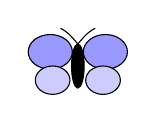
\begin{tikzpicture}[scale=1.0]
% body
\draw[fill=black] (0,0) ellipse (0.08 and 0.28);
% upper wings
\draw[fill=blue!40] (-0.35,0.18) ellipse (0.28 and 0.22);
\draw[fill=blue!40] (0.35,0.18) ellipse (0.28 and 0.22);
% lower wings
\draw[fill=blue!20] (-0.32,-0.18) ellipse (0.22 and 0.18);
\draw[fill=blue!20] (0.32,-0.18) ellipse (0.22 and 0.18);
% antennae
\draw[black] (0,0.28) .. controls (-0.12,0.42) .. (-0.22,0.48);
\draw[black] (0,0.28) .. controls (0.12,0.42) .. (0.22,0.48);
\end{tikzpicture}
};

% Xu box
\node[xu, below=3.3cm of interact.center] (xu)
{\textbf{Competition emerges via shared resource use}\\
Pollinators share nectar 
\\ Plants share pollination\\[1.5pt]};


% Eco–evolutionary feedback loops
\draw[feedback] (fitP.west) to[out=210,in=210,looseness=0.7] (plants.south);
\draw[feedback] (fitA.east) to[out=30,in= -25,looseness=0.7] (polls.south);

\draw[arrow] (plants.south) -- (fitP.north);
\draw[arrow] (polls.south) -- (fitA.north);
\draw[arrow] (fitP.east) -- (xu.west);
\draw[arrow] (fitA.west) -- (xu.east);
\draw[arrow] (plants.north) -- (interact.south west);
\draw[arrow] (polls.north) -- (interact.south east);
% Outer frame
\node[
    draw=black,
    thick,
    rounded corners=4mm,
    fit=(title)(interact)(plants)(polls)(fitP)(fitA)(xu),
    inner sep=8pt
] {};

\end{tikzpicture}

\caption{Conceptual structure of the two-guild mutualistic extension.}
\end{figure}

Note that we in Eq. \ref{pop_dyn_P} we have assumed that the growth factor (i.e. the exponential term) depends only on the mean traits of the plants and pollinators. However, we should in fact calculate the mean growth factor, i.e. the growth factor in Eq. \ref{pop_dyn_P} integrated with respect to the normal distributions of the plant and pollinator traits. This is, for one plant and one animal species,

\begin{align}
\int^\infty_{-\infty} \int^\infty_{-\infty} e^{r_{P} + B_{P}(x_P,y_A) - C_{P}(x_P,y_A) - m_{P} P_{t}} N(x_P) N(y_A) dx_P dy_A   
\end{align}

This is a difficult integral. One way to approximate it is to Taylor expand the integrand. In fact, Eq. \ref{pop_dyn_P} contains the zero-th order term by simply replacing $x_P$ and $y_A$ by the plant and animal mean traits. A first order approximation may already be an improvement.
\end{document}
